\documentclass[a4paper,12pt,twocolumn]{article}
\usepackage[utf8]{inputenc}
\usepackage{graphicx}
\usepackage{hyperref}
\usepackage{comment}

\title{
    Intelligent Control and Cognitive Systems\\
    \begin{large}
        Coursework 1 Report
    \end{large}
}
\author{Adam Jaamour & Tom Slattery}
\date{28th February 2019}

\begin{document}
\maketitle
\thispagestyle{empty}
\clearpage
\setcounter{page}{1}

% ----------------------------------------------------------------------------

\section{Introduction}

The robot is built using the LEGO Mindstorm EV3 kit. Three sensors are used to allow the robot to analyse its environment: two touch sensors and one ultra sonic sensor, along with three motors that provide movement: two large motors for the wheels and one medium motor for the ultra sonic sensor's direction.

\begin{comment}
Todo:
\begin{itemize}
    \item state goal of research
    \item state the different types of sensors used, design reasons (positioning of the sensors for better/optimal readings)
    \item include picture of the robot?
    \item specify approaches using references
    \begin{itemize}
        \item reactive approach using subsumption architecture (Wooldridge, 2009)
        \item --> to allow rover to determine its current situation
        \item using subsumption based on (Brooks, 1991) thesis
    \end{itemize}
\end{itemize}
\end{comment}

% ----------------------------------------------------------------------------

\section{Approach}
The EV3 rover was designed following the simple reflex agent architecture  \cite{brooks1991intelligence}

The rover has three main states which it can transition between.
\begin{itemize}
    \item Initial State
    \item Searching
    \item Wall Following
\end{itemize}
    
Two types of sensors are used to allow the rover to collect data about the environment. A pair of EV3 Touch Sensors are mounted on the front of the rover. They are responsible for detecting collisions with walls. A bar connects the two sensors, with a collision being detected as a response from either sensor. An Ultrasonic depth sensor is used in the "searching" state, once the depth sensor has been triggered. The possible configurations of the position of the robot in relation to the world have been reduced to states observable by the Ultrasonic sensor looking to the left and to the right. 

Experimental Procedure

The rover is placed in an arena, consisting of several fully enclosing walls. The robot begins from a designated starting point. The shape of the arena is preserved between trials.
A single trial consists of a full lap of the arena, returning to the starting point. 





\begin{comment}
Todo:
\begin{itemize}
    \item initial design of rover is usually a simple reflex agent (Russell et al., 1995), allows rover to react to state CRASH but no context for recovery is provided
    \item final design: model-based reflex agent (Russell et al., 1995) allows sensors to modify state
    \item explain how sensor reading quality is improved: take multiple readings at once, if readings are outside the bounds of standard deviation from mean, then not considered. Then the remaining readings are averaged to get final reading that the sensors will act on.
    \item include a perception architecture figure?
    \item explain the decision loops and how they affect/set states (describe the states)
    \item describe rover rates of measurements per second
    \item end by formulating hypothesis e.g. "the rover will perform better if threshold is higher, or if measurements per second is higher, or if 
    \item describe the experiment procedure and conditions (e.g. if robot is stuck then restart experiment)
    \item figure showing layout of the track/obstacles?
    \item mention who did what in the rover's design
    \item mention how morphology helps (wings can help it turn in corners)
    \item motor overcompensating
\end{itemize}

Chosen experience: how modifying the ultrasonic threshold affects lap times and the number of times the touch sensors are used.
Values to test for: [0.01, 0.10, 0.15, 0.20, 0.40, 0.60, 0.80, 1.00]
3 laps per test, average lap times
\end{comment}

\begin{figure*}[ht]
\centering
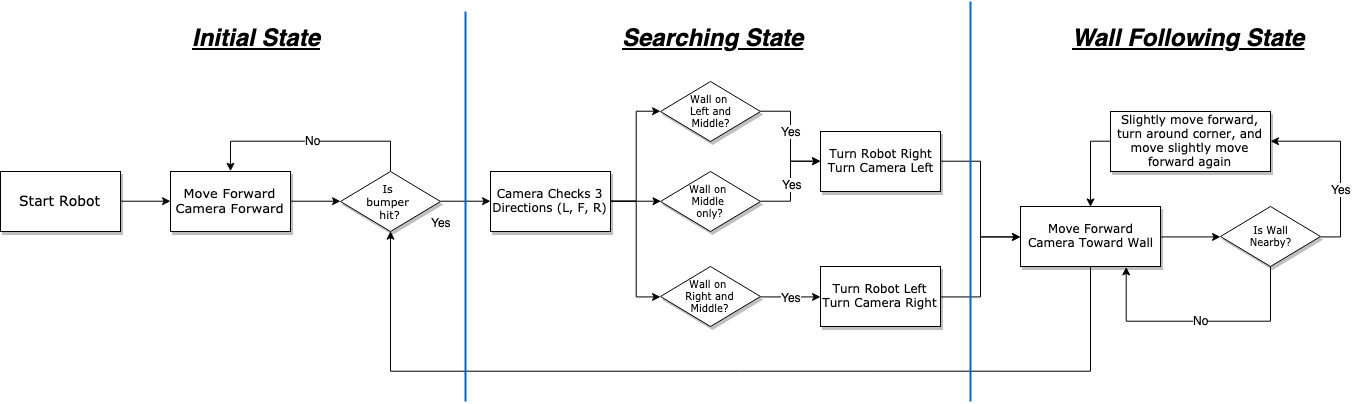
\includegraphics[width=\linewidth]{figures/System-Flowchart.png}
\caption{Flowchart}
  \label{fig:flowchart}
\end{figure*}

% ----------------------------------------------------------------------------

\section{Results}

\begin{comment}
Todo:
\begin{itemize}
    \item state that results are in line with the hypothesis
    \item place results in table
    \item provide link to youtube video
\end{itemize}
\end{comment}

% ----------------------------------------------------------------------------

\section{Discussion}

\begin{comment}
Todo:
\begin{itemize}
    \item suggest improvements (better quality sensors with less noise? more sensors?)
    \item make arena as consistent as possible (obstacles, wall placement, lighting)
\end{itemize}
\end{comment}

% ----------------------------------------------------------------------------

\section{Conclusion}

\begin{comment}
Todo:
\begin{itemize}
    \item single paragraph
    \item what this research set out to do and the results of the research
\end{itemize}
\end{comment}

% ----------------------------------------------------------------------------

\clearpage
\bibliographystyle{plainnat}
\bibliography{bibliography}

\end{document}